% Codigo das figuras desenhadas no proprio LaTeX (TikZ/pgfplots).
% Figura 1 (fig:fluxo): etapas da abordagem sequencial.
% Figura de utilizacao (fig:utilizacao): populacao atendida x capacidade das eSF por UBS no plano.
% Compilar com: xelatex graficos_tikz.tex  (ou pdflatex). Cada figura sai numa pagina do PDF.
\documentclass[tikz,border=8pt]{standalone}
\usepackage[utf8]{inputenc}
\usepackage[T1]{fontenc}
\usetikzlibrary{positioning,arrows.meta,patterns}
\usepackage{pgfplots}
\pgfplotsset{compat=1.16}
\begin{document}

% ---------------- Figura 1: fluxo da abordagem ----------------
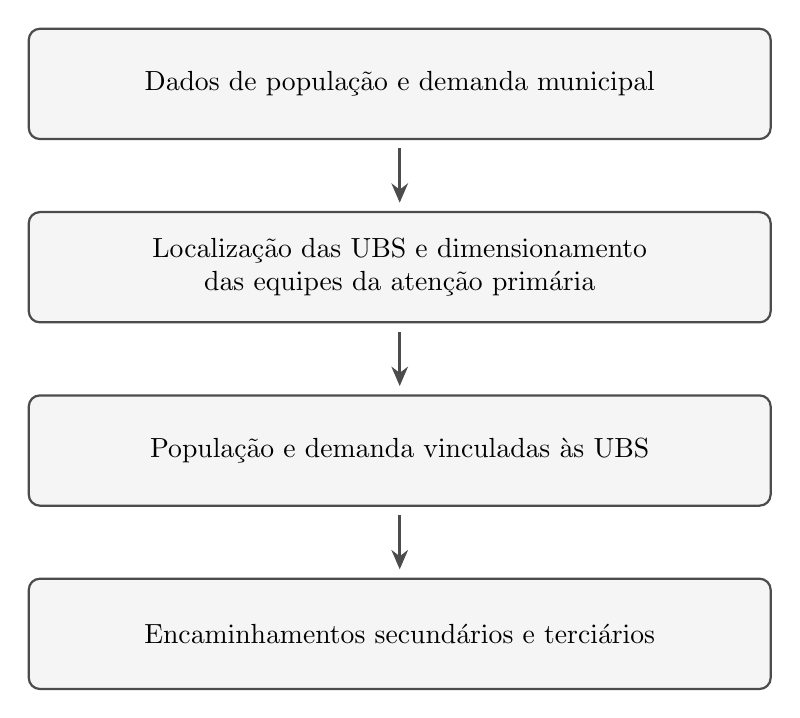
\begin{tikzpicture}[
  etapa/.style={draw=black!70, line width=0.8pt, rounded corners=4pt, fill=black!4,
    text width=9cm, minimum height=1.4cm, align=center, inner sep=6pt, font=\normalsize},
  seta/.style={-{Stealth[length=7pt,width=6pt]}, line width=0.9pt, black!70,
    shorten >=3pt, shorten <=3pt},
  node distance=0.9cm]
\node[etapa] (dados) {Dados de população e demanda municipal};
\node[etapa, below=of dados] (aps) {Localização das UBS e dimensionamento\\ das equipes da atenção primária};
\node[etapa, below=of aps] (vinc) {População e demanda vinculadas às UBS};
\node[etapa, below=of vinc] (enc) {Encaminhamentos secundários e terciários};
\draw[seta] (dados.south) -- (aps.north);
\draw[seta] (aps.south) -- (vinc.north);
\draw[seta] (vinc.south) -- (enc.north);
\end{tikzpicture}

% ---------------- Figura: utilizacao das UBS no plano ----------------
% Barras hachuradas = capacidade (3.000 hab. por eSF); verde = UBS existente; vermelho = nova UBS (N1 a N9).
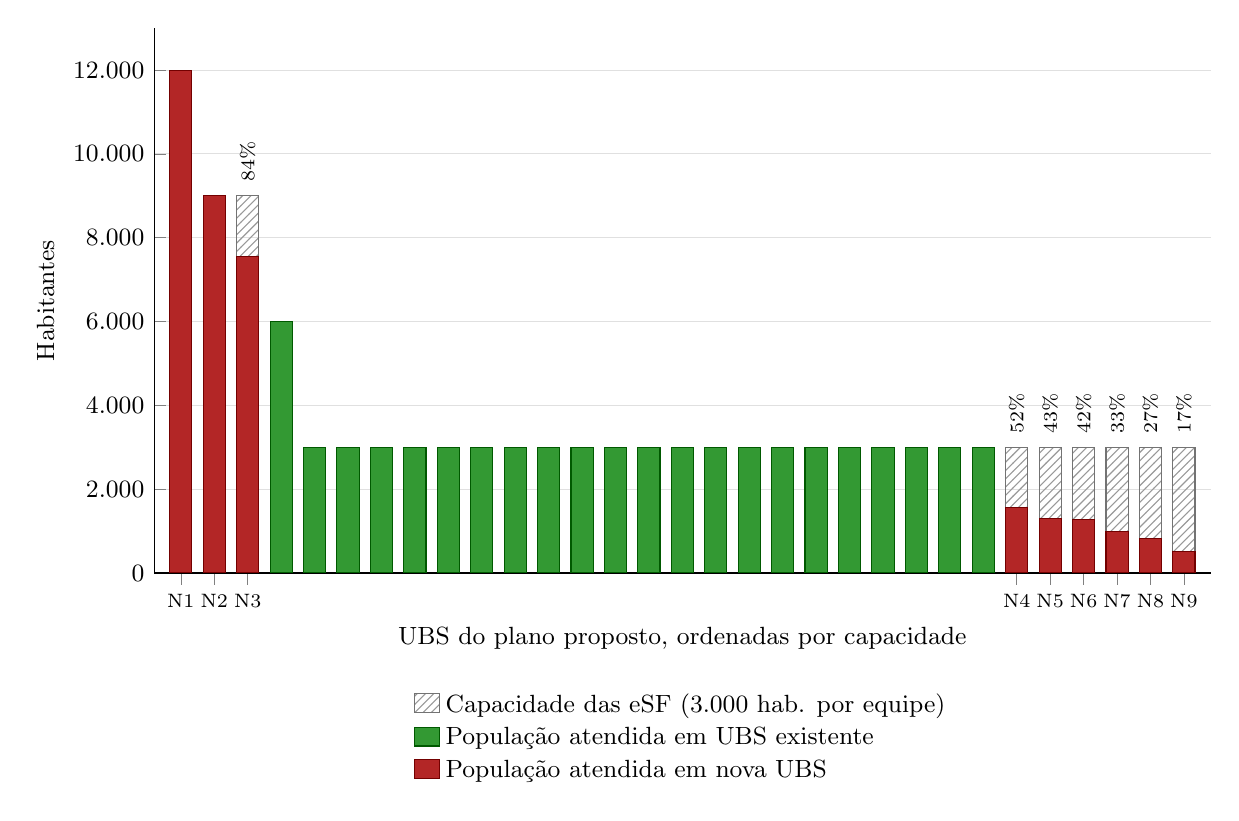
\begin{tikzpicture}
\begin{axis}[
  ybar, bar shift=0pt, bar width=8pt, width=15cm, height=8.5cm,
  xmin=0.2, xmax=31.8, ymin=0, ymax=13000,
  axis y line*=left, axis x line*=bottom,
  ylabel={Habitantes}, ylabel style={font=\small},
  xlabel={UBS do plano proposto, ordenadas por capacidade}, xlabel style={font=\small},
  yticklabel style={font=\small, /pgf/number format/.cd, 1000 sep={.}},
  scaled y ticks=false, ytick={0,2000,4000,6000,8000,10000,12000},
  xtick={1,2,3,26,27,28,29,30,31},
  xticklabels={N1,N2,N3,N4,N5,N6,N7,N8,N9},
  xticklabel style={font=\scriptsize},
  ymajorgrids, grid style={black!12},
  legend style={at={(0.5,-0.2)}, anchor=north, legend columns=1, legend cell align=left, draw=none, font=\small,
    /tikz/every even column/.append style={column sep=12pt}},
  legend image code/.code={\draw[#1] (0cm,-0.1cm) rectangle (0.32cm,0.14cm);},
]
\addplot[draw=black!55, fill=white, pattern=north east lines, pattern color=black!40] coordinates {(1,12000) (2,9000) (3,9000) (4,6000) (5,3000) (6,3000) (7,3000) (8,3000) (9,3000) (10,3000) (11,3000) (12,3000) (13,3000) (14,3000) (15,3000) (16,3000) (17,3000) (18,3000) (19,3000) (20,3000) (21,3000) (22,3000) (23,3000) (24,3000) (25,3000) (26,3000) (27,3000) (28,3000) (29,3000) (30,3000) (31,3000)};
\addplot[draw=green!35!black, fill=green!50!black!80] coordinates {(4,6000) (5,3000) (6,3000) (7,3000) (8,3000) (9,3000) (10,3000) (11,3000) (12,3000) (13,3000) (14,3000) (15,3000) (16,3000) (17,3000) (18,3000) (19,3000) (20,3000) (21,3000) (22,3000) (23,3000) (24,3000) (25,3000)};
\addplot[draw=red!45!black, fill=red!65!black!85] coordinates {(1,12000) (2,9000) (3,7560) (26,1553) (27,1297) (28,1267) (29,985) (30,821) (31,520)};
\legend{Capacidade das eSF (3.000 hab. por equipe), População atendida em UBS existente, População atendida em nova UBS}
\node[font=\scriptsize, rotate=90, anchor=west] at (axis cs:3,9100) {84\%};
\node[font=\scriptsize, rotate=90, anchor=west] at (axis cs:26,3100) {52\%};
\node[font=\scriptsize, rotate=90, anchor=west] at (axis cs:27,3100) {43\%};
\node[font=\scriptsize, rotate=90, anchor=west] at (axis cs:28,3100) {42\%};
\node[font=\scriptsize, rotate=90, anchor=west] at (axis cs:29,3100) {33\%};
\node[font=\scriptsize, rotate=90, anchor=west] at (axis cs:30,3100) {27\%};
\node[font=\scriptsize, rotate=90, anchor=west] at (axis cs:31,3100) {17\%};
\end{axis}
\end{tikzpicture}

\end{document}
